\documentclass[12pt]{article}
\usepackage[utf8]{inputenc}
\usepackage[T1]{fontenc}
\usepackage{fontspec}
\setmainfont{Times New Roman}
\newfontfamily\hackfont{Hack}
\usepackage{titlesec}
\usepackage{fancyhdr}
\usepackage{listings}
\usepackage{xcolor}
\usepackage{graphicx}
\usepackage{longtable}
\usepackage{caption}
\usepackage{hyperref}
\usepackage{setspace}
\usepackage{geometry}
\geometry{a4paper, margin=1in}
\hypersetup{colorlinks=true, linkcolor=blue, urlcolor=blue}
\renewcommand{\contentsname}{Table of Contents}



\begin{document}

\begin{titlepage}					% Cover Start
\begin{center}
    
\includegraphics[width=0.35\textwidth]{logo.png} \\
    \vspace{0.5cm}
    \textbf{\Huge \textcolor{cyan}{NOTRE DAME} \textcolor{cyan}{UNIVERSITY}} \\
    \vspace{0.5cm}
    \textbf{\Huge \textcolor{orange}{BANGLADESH}} \\
    
    \vspace{0.9cm}
    \textbf{\Huge \underline{Computer Graphics Project Proposal}} \\
    
    \vspace{1.5em}
    \begin{flushleft}
    	\textbf{\Large Course Code: CSE-4204} \\
		\vspace{0.3cm}        
        \textbf{\Large Course Title: Computer Graphics Lab} \\
        \vspace{0.3cm}
        \textbf{\Large Project Topic: Egg Drop Game using Glut} \\        
    \end{flushleft}
    
    \vspace{1em}
    \begin{flushleft}
        \textbf{\Huge \textcolor{blue}{Submitted by:}} \\
        \vspace{0.3cm}
        \textbf{\Large Name: Istiak Alam} \\
        \vspace{0.3cm}
        \textbf{\Large ID: 0692230005101005} \\
		\vspace{0.3cm}        
        \textbf{\Large Batch: CSE-20} \\
        \vspace{0.5cm}
        \textbf{\Large Submission Date: }{\Large \textbf{\today}\par}
    \end{flushleft}
    \vfill
    \begin{flushleft}
        \textbf{\Huge \textcolor{blue}{Submitted to:}} \\
        \vspace{0.3cm}
        \textbf{\Large Humayara Binte Rashid} \\
        \vspace{0.3cm}
        \textbf{\Large Lecturer, Dept. of CSE} \\
        \vspace{0.3cm}
        \textbf{\Large Notre Dame University Bangladesh}
    \end{flushleft}
\end{center}
\end{titlepage}						% Cover End



\rfoot{\thepage}
\tableofcontents						% Table of contents
\thispagestyle{empty}
\clearpage
\pagenumbering{arabic}
\pagestyle{fancy}
\fancyhf{} 							% Header Middle
\rhead{Computer Graphics}
\lhead{Project Report-01}

%							PAGE START


\section{Project Proposal Description}

\subsection{Project Title}
\textbf{Egg Drop Saga Using OpenGL Glut}

\subsection{Introduction}

Computer graphics plays an important role in modern software applications, particularly in the development of interactive games and visual simulations. This project proposes the development of a simple yet engaging 2D game called \textit{Egg Drop Saga Game}. The game will be developed using the C++ programming language along with the OpenGL graphics library and GLUT toolkit for rendering graphics and handling user input.

The objective of the game is to create an interactive environment where a player controls a bucket to catch eggs dropped by a chicken positioned at the top of the screen. The player must move the bucket left or right to successfully catch falling eggs while avoiding missed eggs.

\subsection{Objectives}

The main objectives of this project are:

\begin{itemize}
\item To design and implement a 2D interactive game using OpenGL.
\item To demonstrate the use of computer graphics primitives such as shapes, colors, and transformations.
\item To implement animation techniques for moving objects within the game.
\item To apply collision detection between game objects.
\item To create a simple but engaging user experience.
\end{itemize}

\subsection{Project Overview}

The game environment consists of three main graphical elements:

\begin{itemize}
\item \textbf{Chicken}: Positioned at the top of the screen, the chicken periodically lays eggs.
\item \textbf{Egg}: Eggs fall from the chicken toward the bottom of the screen with a certain speed.
\item \textbf{Bucket}: Controlled by the player to catch the falling eggs.
\end{itemize}

The player will use keyboard input (left and right arrow keys) to move the bucket horizontally across the screen. If the bucket successfully catches an egg, the player receives a score point. If the egg reaches the ground without being caught, the player loses a life or score opportunity.

\section{Graphical Analysis}

This section presents graphical analysis related to the performance or behavior of the Egg Catching Game. The graph illustrates important aspects such as gameplay performance, score progression, or object movement patterns during gameplay. The graph is included as a PDF figure for better visualization and analysis.

\subsection{Graph Representation}

The following figure shows the graphical representation used in this project.

\begin{figure}[h]
    \centering
    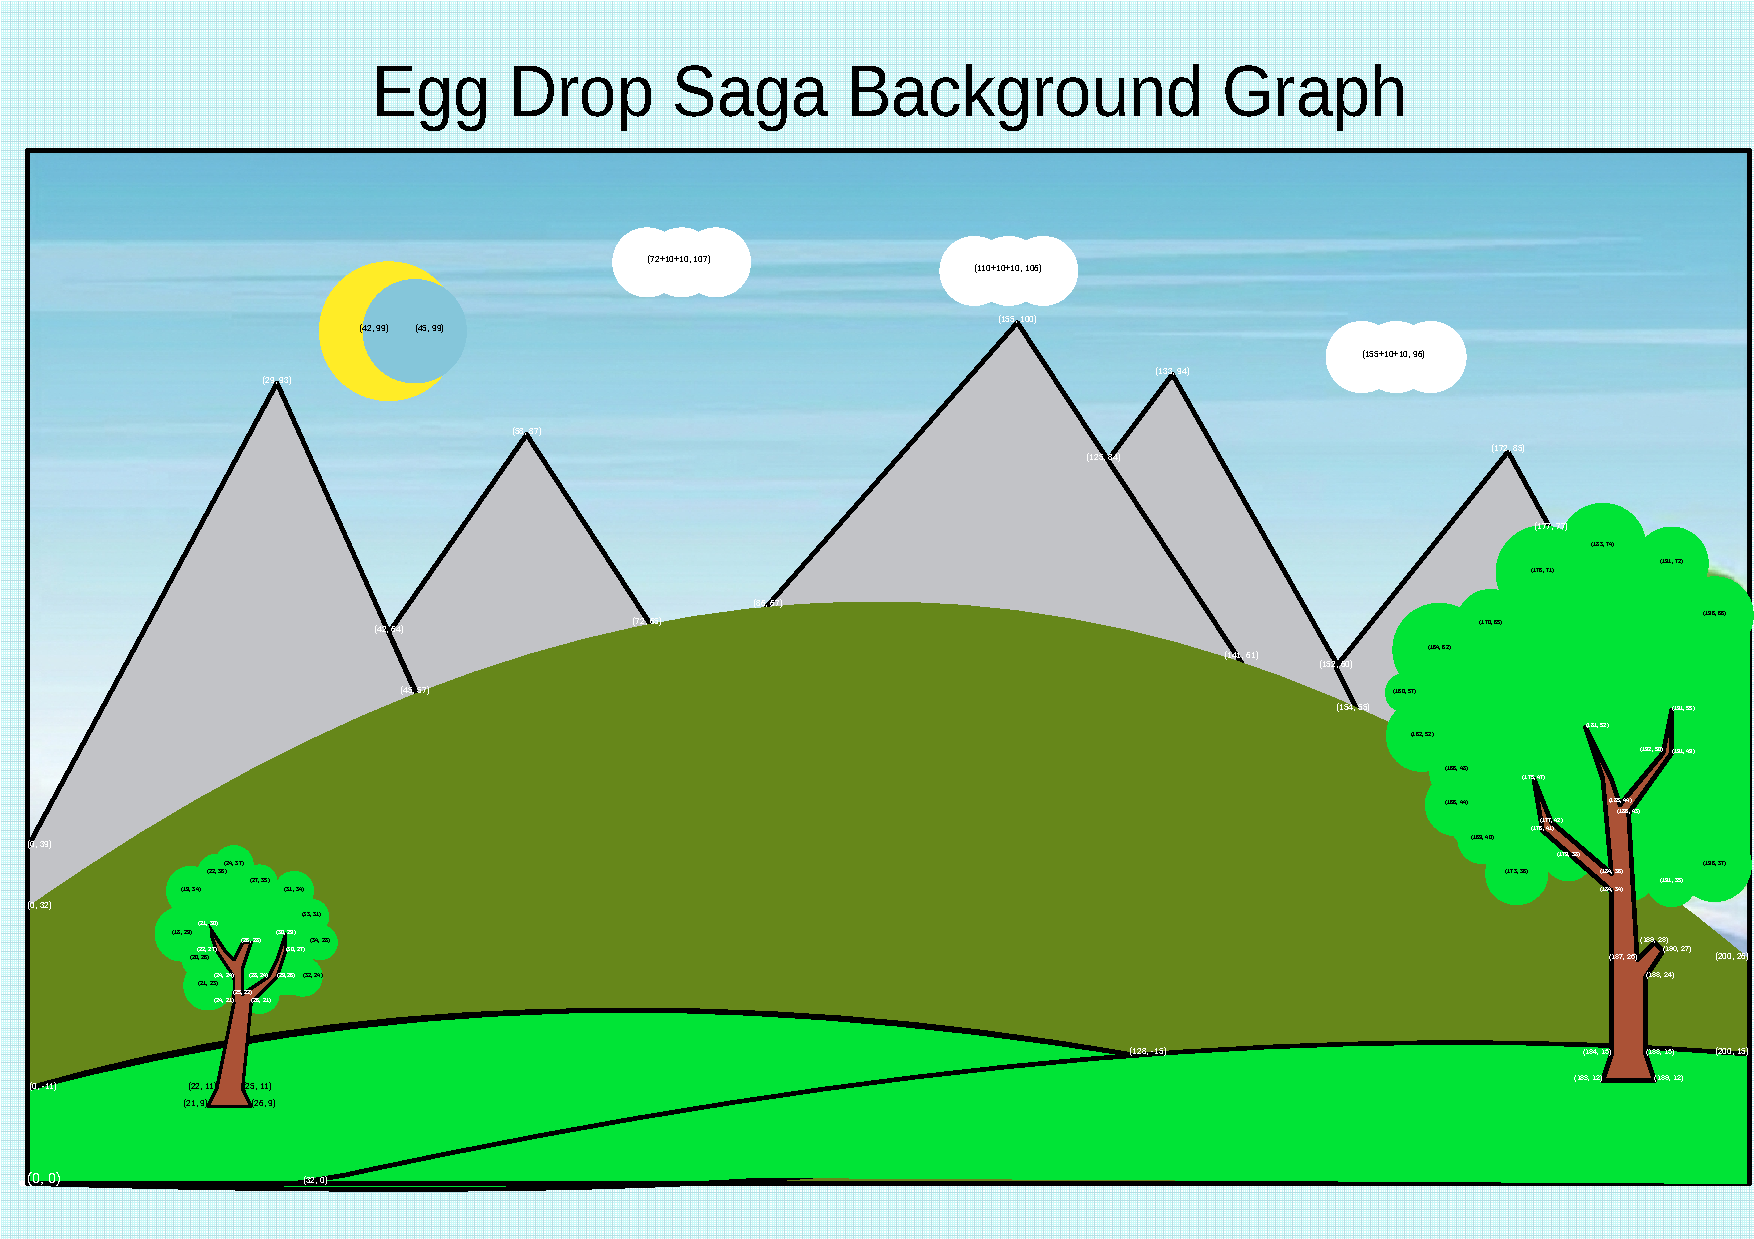
\includegraphics[width=0.8\textwidth]{graph.pdf}
    \caption{Target Background Graph of the Egg Drop Saga Game}
    \label{fig:game_graph}
\end{figure}

\subsection{Graph Source}

The graph used in this report can be accessed from the following resources:

\begin{itemize}
    \item PDF File: \href{graph.pdf}{Open Graph PDF}
    \item Online Link: \href{https://virtual-graph-paper.com/ZDNjOTYyYmUxY2Nj}{Graph Source Link}
\end{itemize}

\subsection{Graph Description}

The graph demonstrates the relationship between different gameplay parameters such as time, score, or egg spawn rate. It helps in analyzing how the game behaves during execution and provides insights into gameplay dynamics and performance.

This analysis is useful for understanding game mechanics and evaluating the effectiveness of the implemented graphics and animation logic.

\subsection{Graphics Implementation}

The project uses OpenGL primitives such as:

\begin{itemize}
\item \textbf{GL\_TRIANGLE\_FAN} for drawing circular shapes like eggs and the chicken body.
\item \textbf{GL\_QUADS} for drawing the bucket.
\item Basic color shading to represent different game objects.
\end{itemize}

The animation is implemented through continuous screen updates using the rendering loop. The egg's vertical position is updated over time to simulate gravity and falling motion.

\subsection{Collision Detection}

A collision detection mechanism is implemented to determine when an egg intersects with the bucket. This is achieved using a simple bounding box or positional comparison between the coordinates of the egg and the bucket. When a collision occurs, the egg is considered caught and the player's score is updated.

\subsection{Game Mechanics}

The gameplay includes the following mechanics:

\begin{itemize}
\item Eggs are generated periodically at the chicken's position.
\item Eggs fall downward with a constant speed.
\item The player moves the bucket horizontally to catch eggs.
\item If an egg collides with the bucket, it is removed and the score increases.
\item If the egg reaches the bottom of the screen, it is considered missed.
\end{itemize}

\subsection{Expected Outcome}

The final outcome of the project will be a fully functional 2D game demonstrating basic concepts of computer graphics, animation, and interactive gameplay. The project will highlight the practical use of OpenGL for rendering objects, handling animation, and implementing user interaction within a graphical environment.

Additionally, the project will serve as a learning platform for understanding fundamental game development techniques including object rendering, event handling, and collision detection.




\end{document}